%------------------------------------------------------------------------------------
\section{Sensor Kinect}
\subsection{Historia}
El primer anuncio de Kinect fue el 1 de Junio de 2009 en la E3 2009 bajo el nombre de ``Project Natal".\\

Kinect es una línea de dispositivos de detección de movimientos de Microsoft para las consolas de videojuegos Xbox 360 así como para PCs con sistema operativo Windows. Basado en torno a un periférico tipo webcam, permite a los usuarios controlar e interactuar con su consola/computadora sin la necesidad de un control de juego, a través de una interfaz natural de usuario usando gestos y comando de voz \cite{Microsoft2}.\\

Formalmente Microsoft presentó en Junio del 2010 en la E3 que su sistema se llamaría oficialmente Kinect \cite{Snider}.
%------------------------------------------------------------------------------------
\subsection{Descripción del hardware}
El Kinect se compone de una cabeza y de una base, como se muestra en la Figura \ref{fig:Kinect}. La cabeza es de 12 x 2.5 x 1.5 pulgadas. La unión entre la base y la cabeza está motorizada. El dispositivo físico contiene cámaras, una colección de micrófonos y un acelerómetro \cite{Webb}.

\begin{figure}[h]%La h significa que la colocara cerca del texto
	\begin{center}
		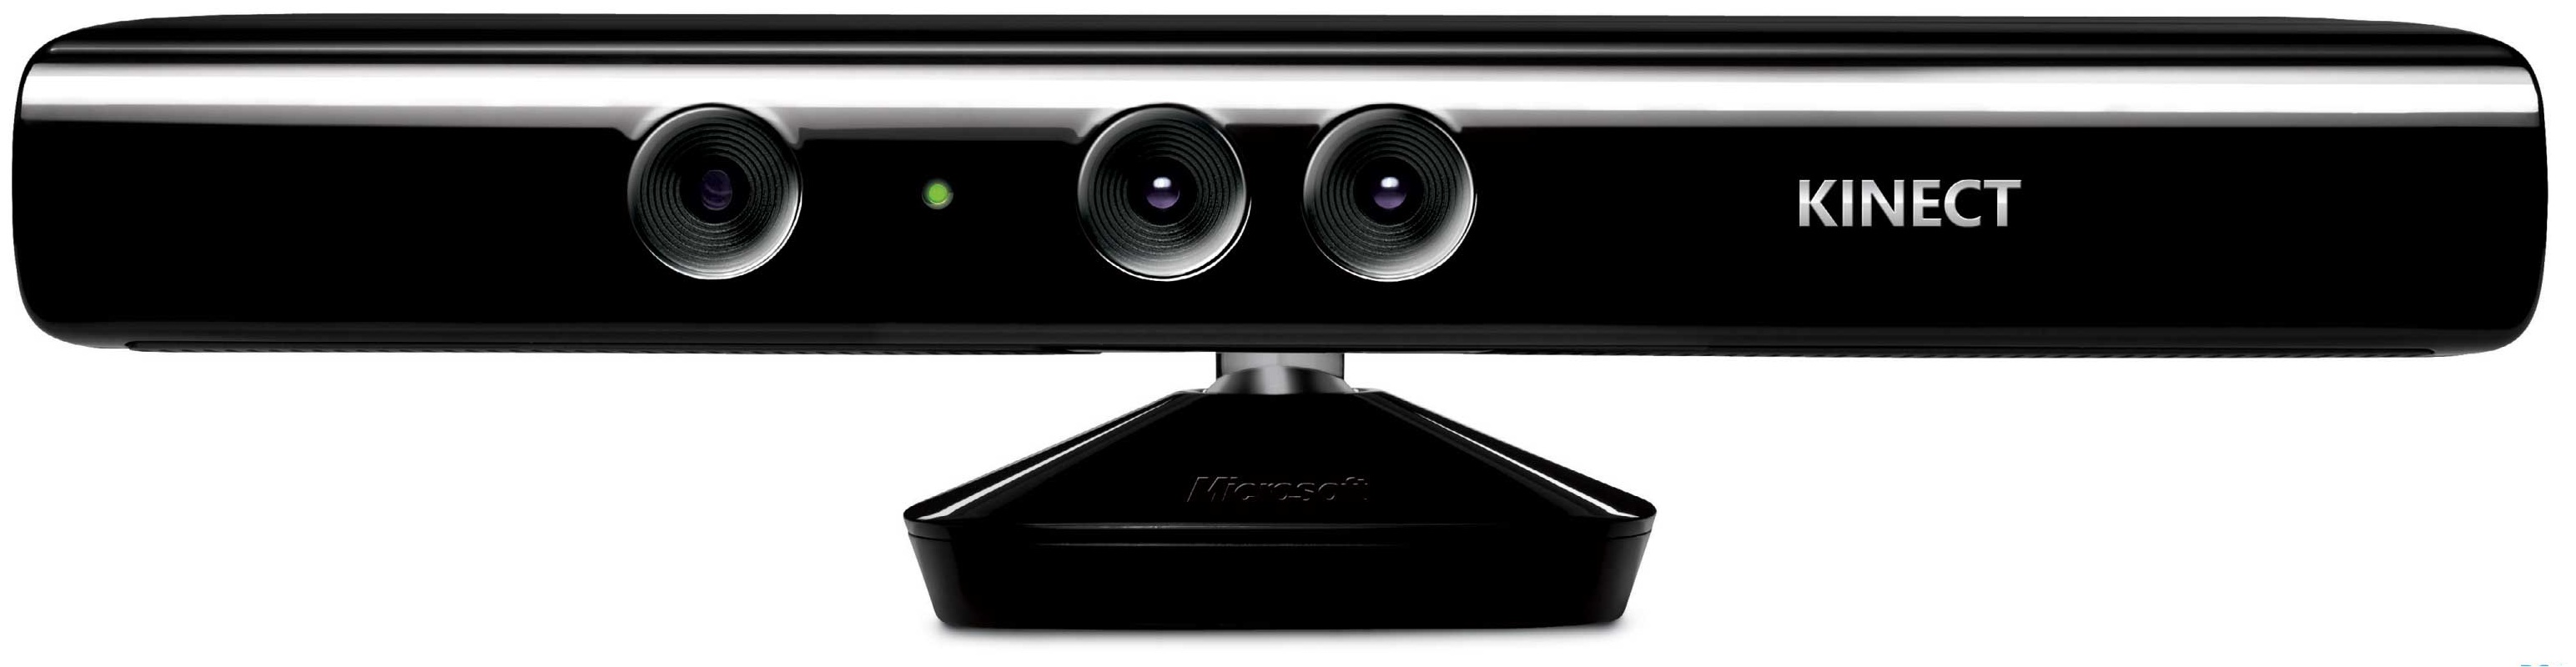
\includegraphics[scale=0.15]{./Figuras/KinectFrontal}
	\end{center}
	\caption{Vista frontal del Kinect}
	\label{fig:Kinect}
\end{figure}

Dentro del recubrimiento del sensor, un Kinect para Windows contiene:

\begin{itemize}
\item Una cámara RGB que almacena 3 canales de datos en una resolución de 1280x960. Esto permite capturar imágenes a color.
\item Un emisor infrarrojo (IR) y un sensor infrarrojo de profundidad. El emisor emite destellos de luz infrarroja y el sensor de profundidad lee los haces de luz infrarroja reflejadas de nuevo al sensor. Los haces reflejados son convertidos en información de profundidad midiendo la distancia entre un objeto y el sensor. Esto permite capturar la profundidad de una imagen.
\item Un micrófono multi-array, el cual contiene 4 micrófonos para capturar sonido. Debido a los 4 micrófonos, es posible grabar audio, así como encontrar la ubicación de la fuente de sonido y la dirección de la onda de audio.
\item Un acelerómetro de 3 ejes configurado para rango 2G donde la G es la aceleración debida a la gravedad. Es posible usar el acelerómetro para determinar la orientación actual del Kinect \cite{Microsoft3}.
\end{itemize}

\begin{figure}[h]%La h significa que la colocara cerca del texto
	\begin{center}
		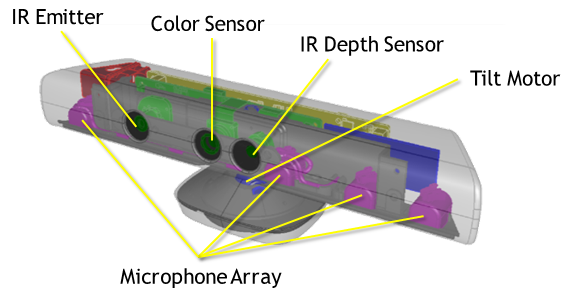
\includegraphics[scale=1]{./Figuras/KinectHardware}
	\end{center}
	\caption{Hardware interno del Kinect}
	\label{fig:KinectHardware}
\end{figure}
%------------------------------------------------------------------------------------
\subsection{Kinect SDK}
Microsoft Kinect SDK, provee las herramientas y API's necesarias para desarrollar aplicaciones para Microsoft Windows usando la tecnología de sensores de Kinect \cite{MicrosoftSDK}.\\

Existen 4 actualizaciones de la versión de SDK para el sensor Kinect, de las cuales la 1.8 es la versión a utilizar en el presente trabajo terminal, algunas características que se tienen hasta el momento son:
\begin{itemize}
\item Kinect Studio: Herramienta que permite a los desarrolladores grabar y reproducir datos de Kinect.
\item Reconocimiento del esqueleto ``sentado": Permite el seguimiento de 10 puntos (cabeza, cuello y brazos) ignorando las piernas y la cintura.
\item Datos ampliados profundidad: Las aplicaciones serán capaces de leer los datos más allá de cuatro metros cuando sea necesario.                                                                                                                  
\item APIs de configuración de la cámara a color: Los ajustes de la cámara de color se pueden optimizar para su entorno.
\item Nueva API de conversión de coordenadas espacio: Hay dos conjuntos de APIs, uno para la conversión de los píxeles individuales y la otra para la conversión de un cuadro de imagen completa.
\item Kinect Interactions: Ofrece la posibilidad a los desarrolladores de crear aplicaciones intuitivas que utilicen los gestos más comunes de la gente.
\item Kinect for Windows Interactions: Transforma la manera en la que la gente se comunica con la computadora.
\item Incluye herramientas de desarrollo mejoradas y más recursos para los desarrolladores tales como: Ejemplos de OpenCV y MATLAB compatibles con Kinect, ejemplos de código de Kinect para Windows para CodePlex ofreciendo la posibilidad de desarrollar en una plataforma open-source \cite{Heddle1}.
\end{itemize} 

Las características principales de la última versión (1.8) incluyen: 
\begin{itemize}
\item Un nuevo efecto de pantalla verde: Permite borrar el fondo detrás del usuario activo y después intercambiarlo por un fondo artificial.
\item Capacidades mejoradas para modelado en 3D: Permiten escanear el color de una escena al igual que sus contornos, lo que hace posible la impresión de objetos en 3D a todo color o pueda agregarse fidelidad a las características de los juegos y otras aplicaciones.
\item Una muestra de interfaz de usuario adaptable: Muestra cómo construir una aplicación que se adapta de acuerdo con la distancia entre el usuario y la pantalla para detección de gestos y tacto \cite{Heddle2}.
\end{itemize}
%------------------------------------------------------------------------------------
\subsection{Kinect SDK Open Source}
\subsubsection{OpenNI (Open Natural Interaction)}
Es un framework de código abierto creado por la empresa PrimeSense, permite comunicarse con los sensores de audio, video y sensor de profundidad de Kinect, mientras que proporciona una API que sirve de puente entre el hardware del equipo, NITE Middleware y las aplicaciones e interfaces del Sistema Operativo.  Su idea es facilitar el desarrollo de aplicaciones que funcionen con interacción natural, como gestos y movimientos corporales \cite{Echeverria}. \\

En noviembre del 2013, Apple compró la empresa PrimeSense. El 23 de abril del 2014, la página de OpenNI cerró y la descarga del software quedó deshabilitada desde esa fecha \cite{Armstrong}.

\subsubsection{OpenKinect}
Su objetivo principal actualmente es el software libfreenect, éste incluye todo el código necesario para activar, inicializar y comunicar los datos con el hardware de Kinect. La API  tiene enlaces y extensiones para los siguientes idiomas y plataformas: C, C++, NET (C\#), Java, Python, C y la interfaz síncrona.\\

OpenKinect también tiene como proyecto, la librería de análisis la cual se comunica con el API y analiza la información en bruto en abstracciones más útiles; así como aplicaciones, que incluyan códigos de ejemplo, demos, o cualquier aplicación que los usuarios quieran compartir.\\

El usuario que contribuya, puede optar por utilizar el proyecto con la licencia Apache 2.0 o licencia GPL v2 \cite{OpenKinect}. 